\section{Аппаратная архитектура тракта поиска}


\begin{figure*}[!t]
    \centering
    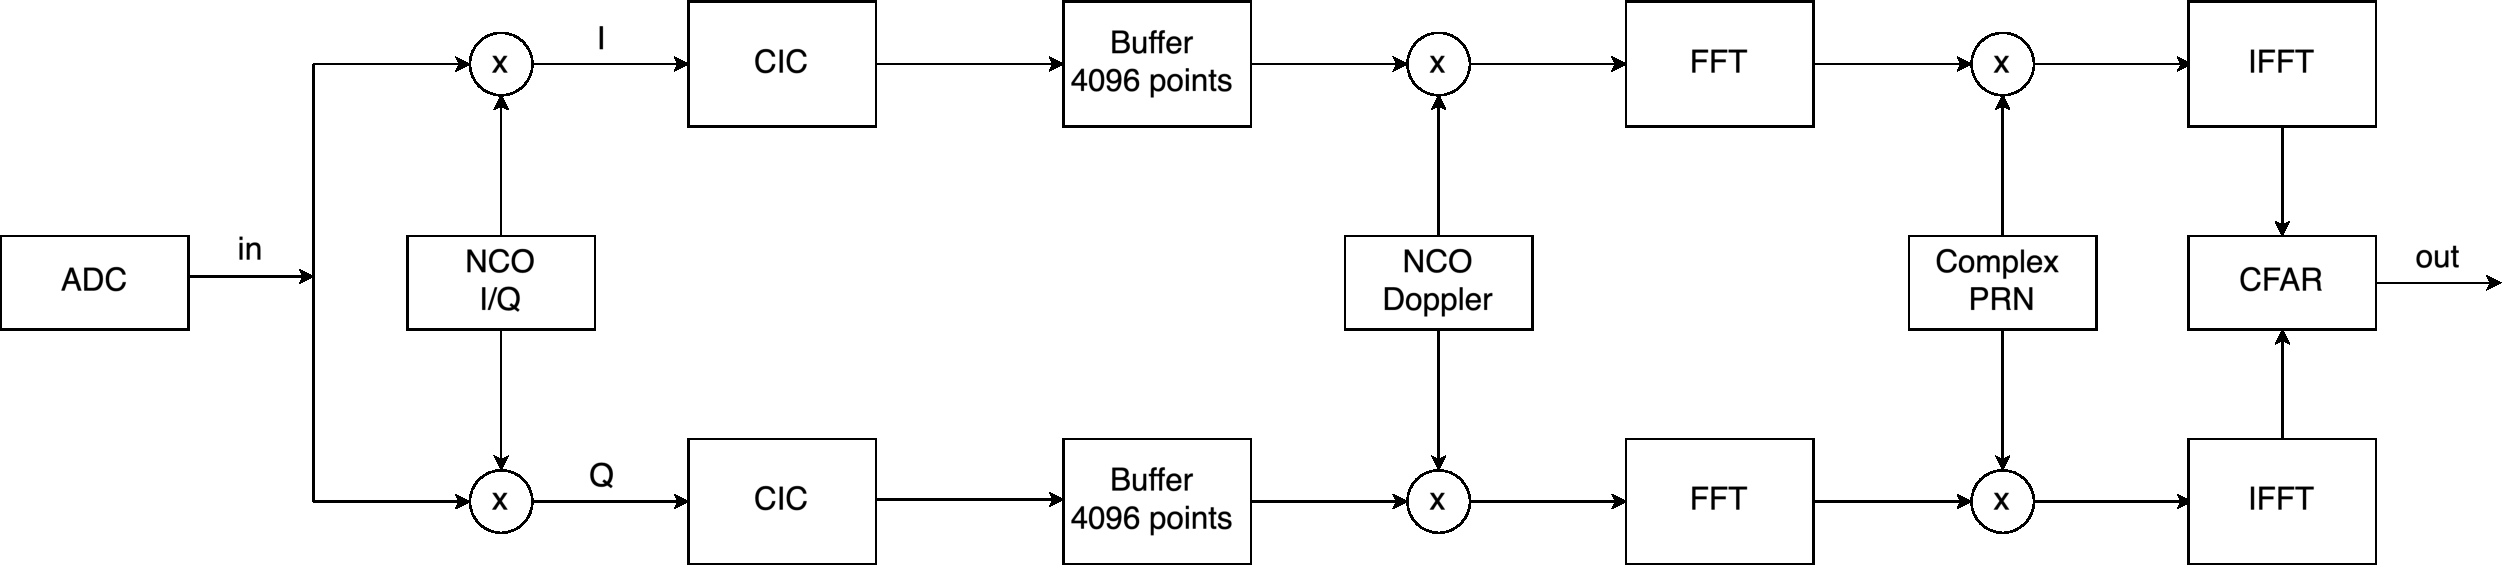
\includegraphics[width=0.9\textwidth]{coarse.pdf}
    \caption{Структурная схема тракта первичного поиска сигналов GPS L1}
    \label{fig:arch}
\end{figure*}

Вычислительный тракт параллельного поиска реализует согласованную фильтрацию входного радиосигнала. Его обобщенная структурная схема представлена на рис.~\ref{fig:arch}. На вход тракта от блока АЦП поступает цифровой поток промежуточной частоты $f_{\text{IF}} = 9{,}548$~МГц при частоте дискретизации $F_s = 38{,}192$~МГц.

\textbf{Квадратурный перенос на нулевую частоту.}
Входной оцифрованный сигнал поступает на блок квадратурного гетеродина (DDC), осуществляющий перенос спектра на нулевую промежуточную частоту путем умножения на отсчеты синусной и косинусной составляющих цифрового генератора:
\begin{equation}
    \begin{cases}
        I[n] = D_{\text{adc}}[n] \cdot \cos(\phi[n]), \\
        Q[n] = D_{\text{adc}}[n] \cdot \sin(\phi[n]).
    \end{cases}
\end{equation}
Поскольку в тракте применен 1-битный АЦП ($D_{\text{adc}}[n] \in \{-1, 1\}$), аппаратная реализация не требует использования многоразрядных умножителей, операция умножения сводится к инверсии знака табличного отсчета NCO в зависимости от текущего бита АЦП.

\textbf{Фильтрация и децимация.}
Сформированные квадратурные компоненты $I[n]$ и $Q[n]$ содержат высокочастотные составляющие спектра на удвоенной промежуточной частоте. Для их подавления и снижения вычислительной нагрузки на последующие блоки тракта применены каскадные интегрально-гребенчатые фильтры (CIC). Модуль осуществляет децимацию входного потока с коэффициентом $R = 10$, понижая исходную частоту дискретизации $F_s = 38{,}192$~МГц до темпа обработки $F_{\text{dec}} = 3{,}8192$~МГц. Выбор CIC-архитектуры обусловлен отсутствием умножителей в ее структуре, что минимизирует площадь кристалла и снижает энергопотребление тракта.

\textbf{Буферизация и дополнение нулями.}
С выхода CIC-фильтров отсчеты квадратурных составляющих поступают в буфер согласования базы. За период повторения дальномерного C/A-кода GPS ($T_{\text{coh}} = 1$~мс) на децимированной частоте $F_{\text{dec}} = 3{,}8192$~МГц накапливается массив из 3819 комплексных отсчетов с точностью до целой части. Для применения radix-2 алгоритма БПФ массив дополняется нулями (zero-padding) до размерности N=4096 отсчётом, при этом уровень наложения циклической корреляции остаётся допустимым и не влияет на положение главного корреляционного пика.

\textbf{Компенсация доплеровского смещения.}
Для устранения частотной неопределенности, вызванной движением космического аппарата, формируется сетка доплеровских гипотез с постоянным шагом $\Delta f_d = 500$~Гц. Перед процедурой спектрального согласованного поиска накопленный в буфере комплексный вектор отсчетов последовательно перемножается на квадратурные составляющие вторичного гетеродина (NCO Doppler), настроенного на соответствующее смещение частоты:
\begin{equation}
    f_{\text{dop}}^{(m)} = m \cdot \Delta f_d, \quad m \in [-M, M],
\end{equation}
где $m$ — номер текущей проверяемой гипотезы. Скомпенсированный во временной области сигнал передается на блок согласованной фильтрации.

\textbf{Согласованная фильтрация и спектральный анализ.}
Для каждой проверенной гипотезы по доплеровскому смещению выполняется процедура быстрого поиска на основе теоремы о свертке. Временной сигнал преобразуется в частотную область с помощью быстрого преобразования Фурье (БПФ), после чего его спектр поэлементно умножается на комплексно сопряженный опорный спектр локального C/A-кода спутника:
\begin{equation}
    Y[k] = X[k] \cdot S^*[k] = (X_I S_I + X_Q S_Q) + j(X_Q S_I - X_I S_Q).
\end{equation}
Затем с помощью обратного преобразования Фурье (ОБПФ) данные возвращаются во временную область, образуя отсчеты автокорреляционной функции. Детальные аппаратные особенности этого конвейера, а также результирующие поверхности отклика будут подробно рассмотрены в следующих разделах работы.

\textbf{Адаптивное пороговое обнаружение.}
Завершающим этапом тракта является блок пороговой обработки по критерию Неймана--Пирсона. На основе квадратов квадратурных составляющих $I^2[k] + Q^2[k]$ модуль формирует двумерную матрицу автокорреляционных откликов в пространстве «задержка--доплеровский сдвиг». Для квадратичного детектора при гауссовом шуме порог, обеспечивающий заданную вероятность ложной тревоги, определяется аналитически:
\begin{equation}
T = -\hat{\sigma}^2 \ln P_{\text{fa}}.
\end{equation}
где вероятность ложной тревоги $P_{\text{fa}} = 10 ^{-5}$.
